%Document class
\documentclass{article}

\usepackage{graphicx}
\usepackage{subfigure}

%Document content
\begin{document}

A continuación se inserta la primera figura.

\begin{figure}[htbp]
  \centering
    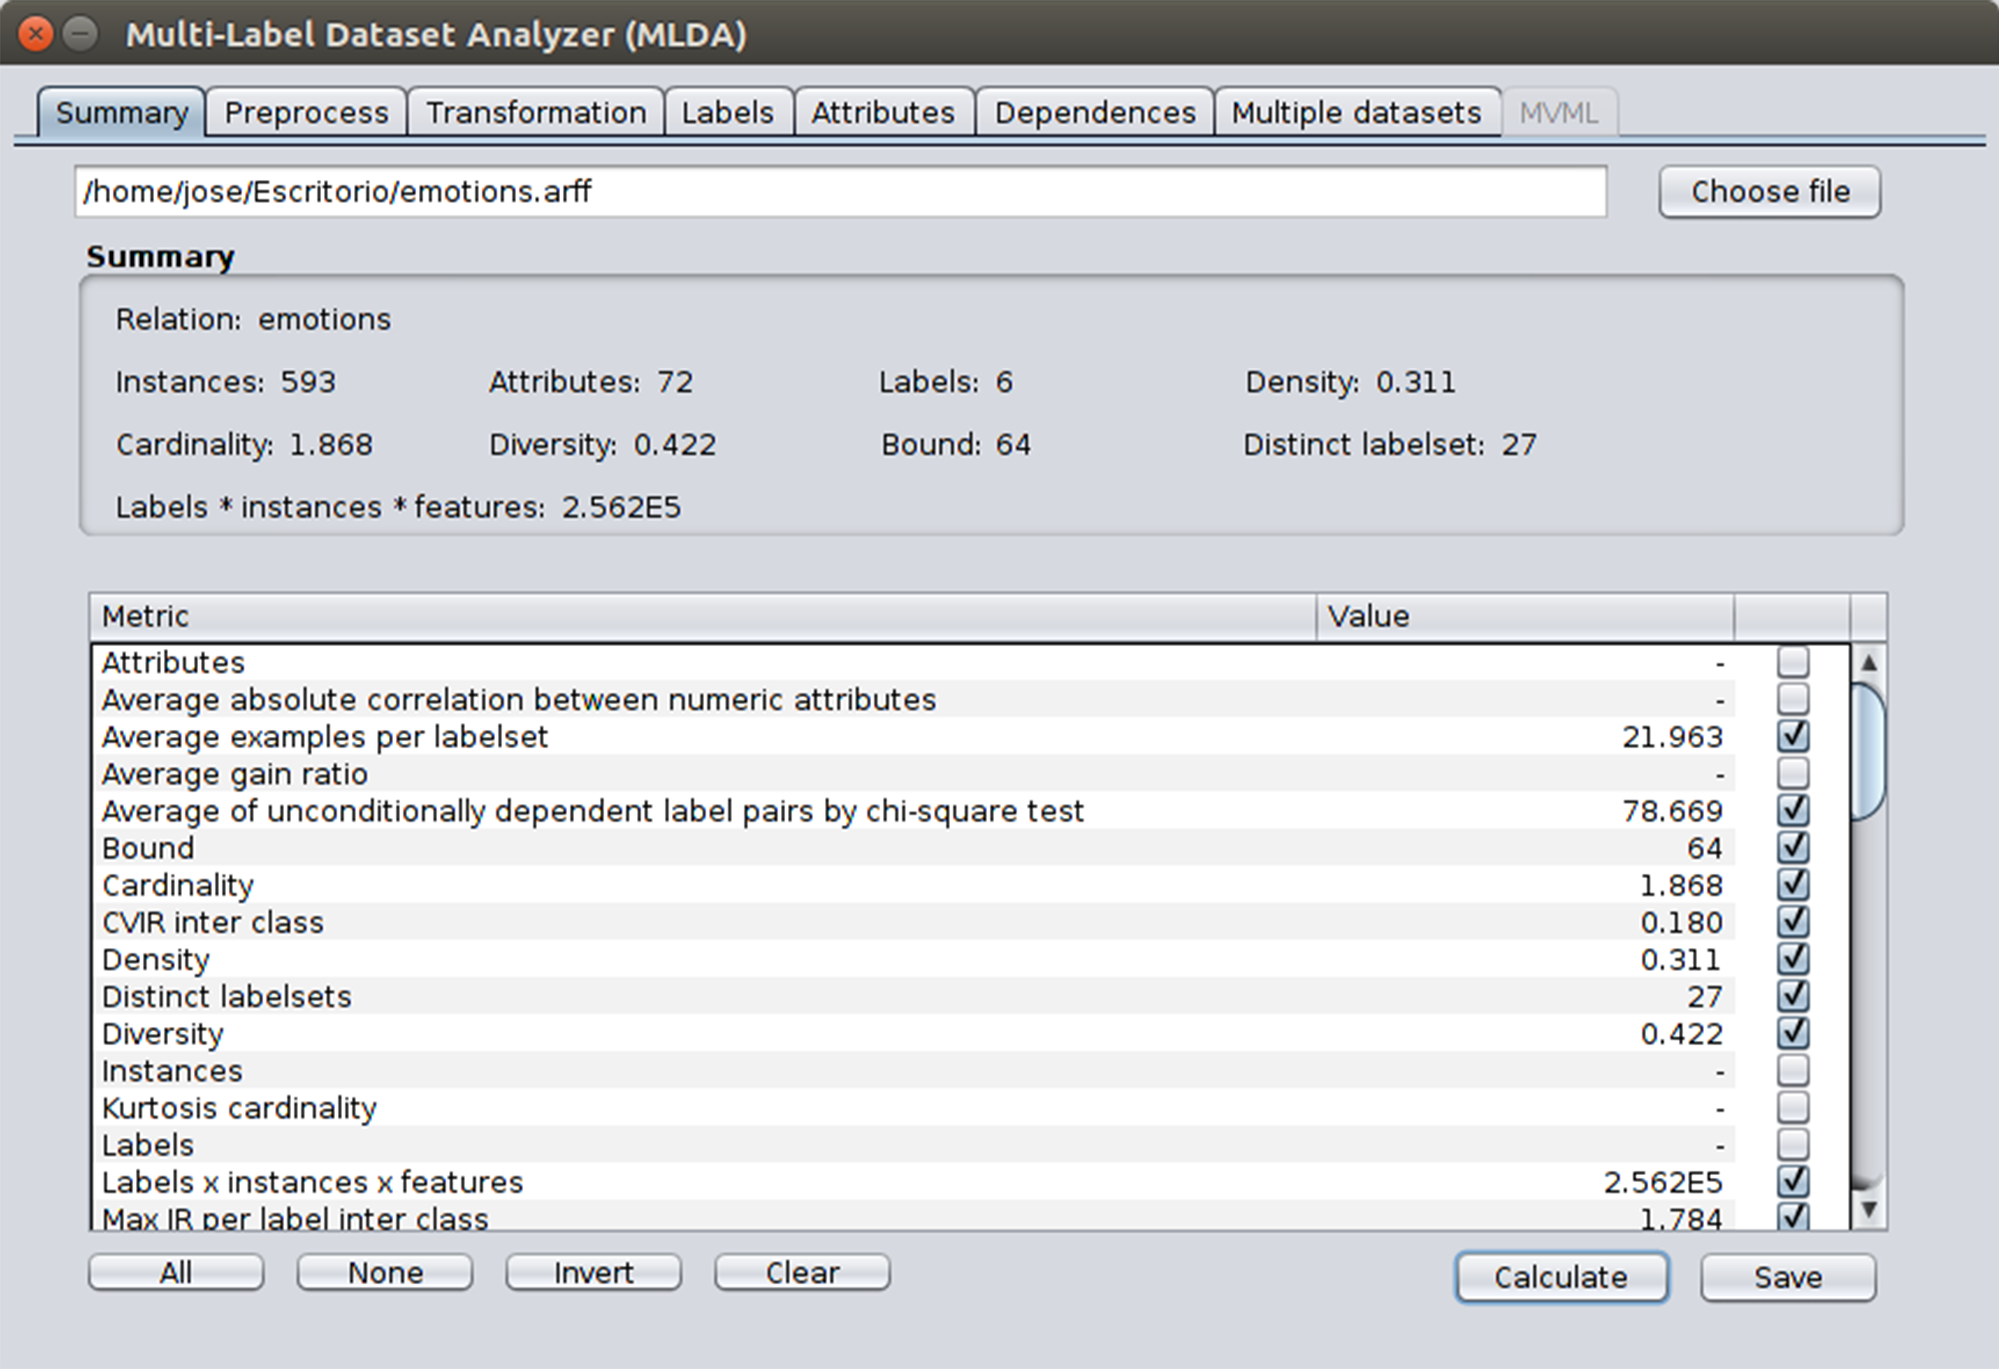
\includegraphics{figs/fig1.png}
  \caption{Mi Figura}
  \label{fig:fig1}
\end{figure}

En la Figura \ref{fig:fig2} se muestra ...

\begin{figure}[htbp]
  \centering
    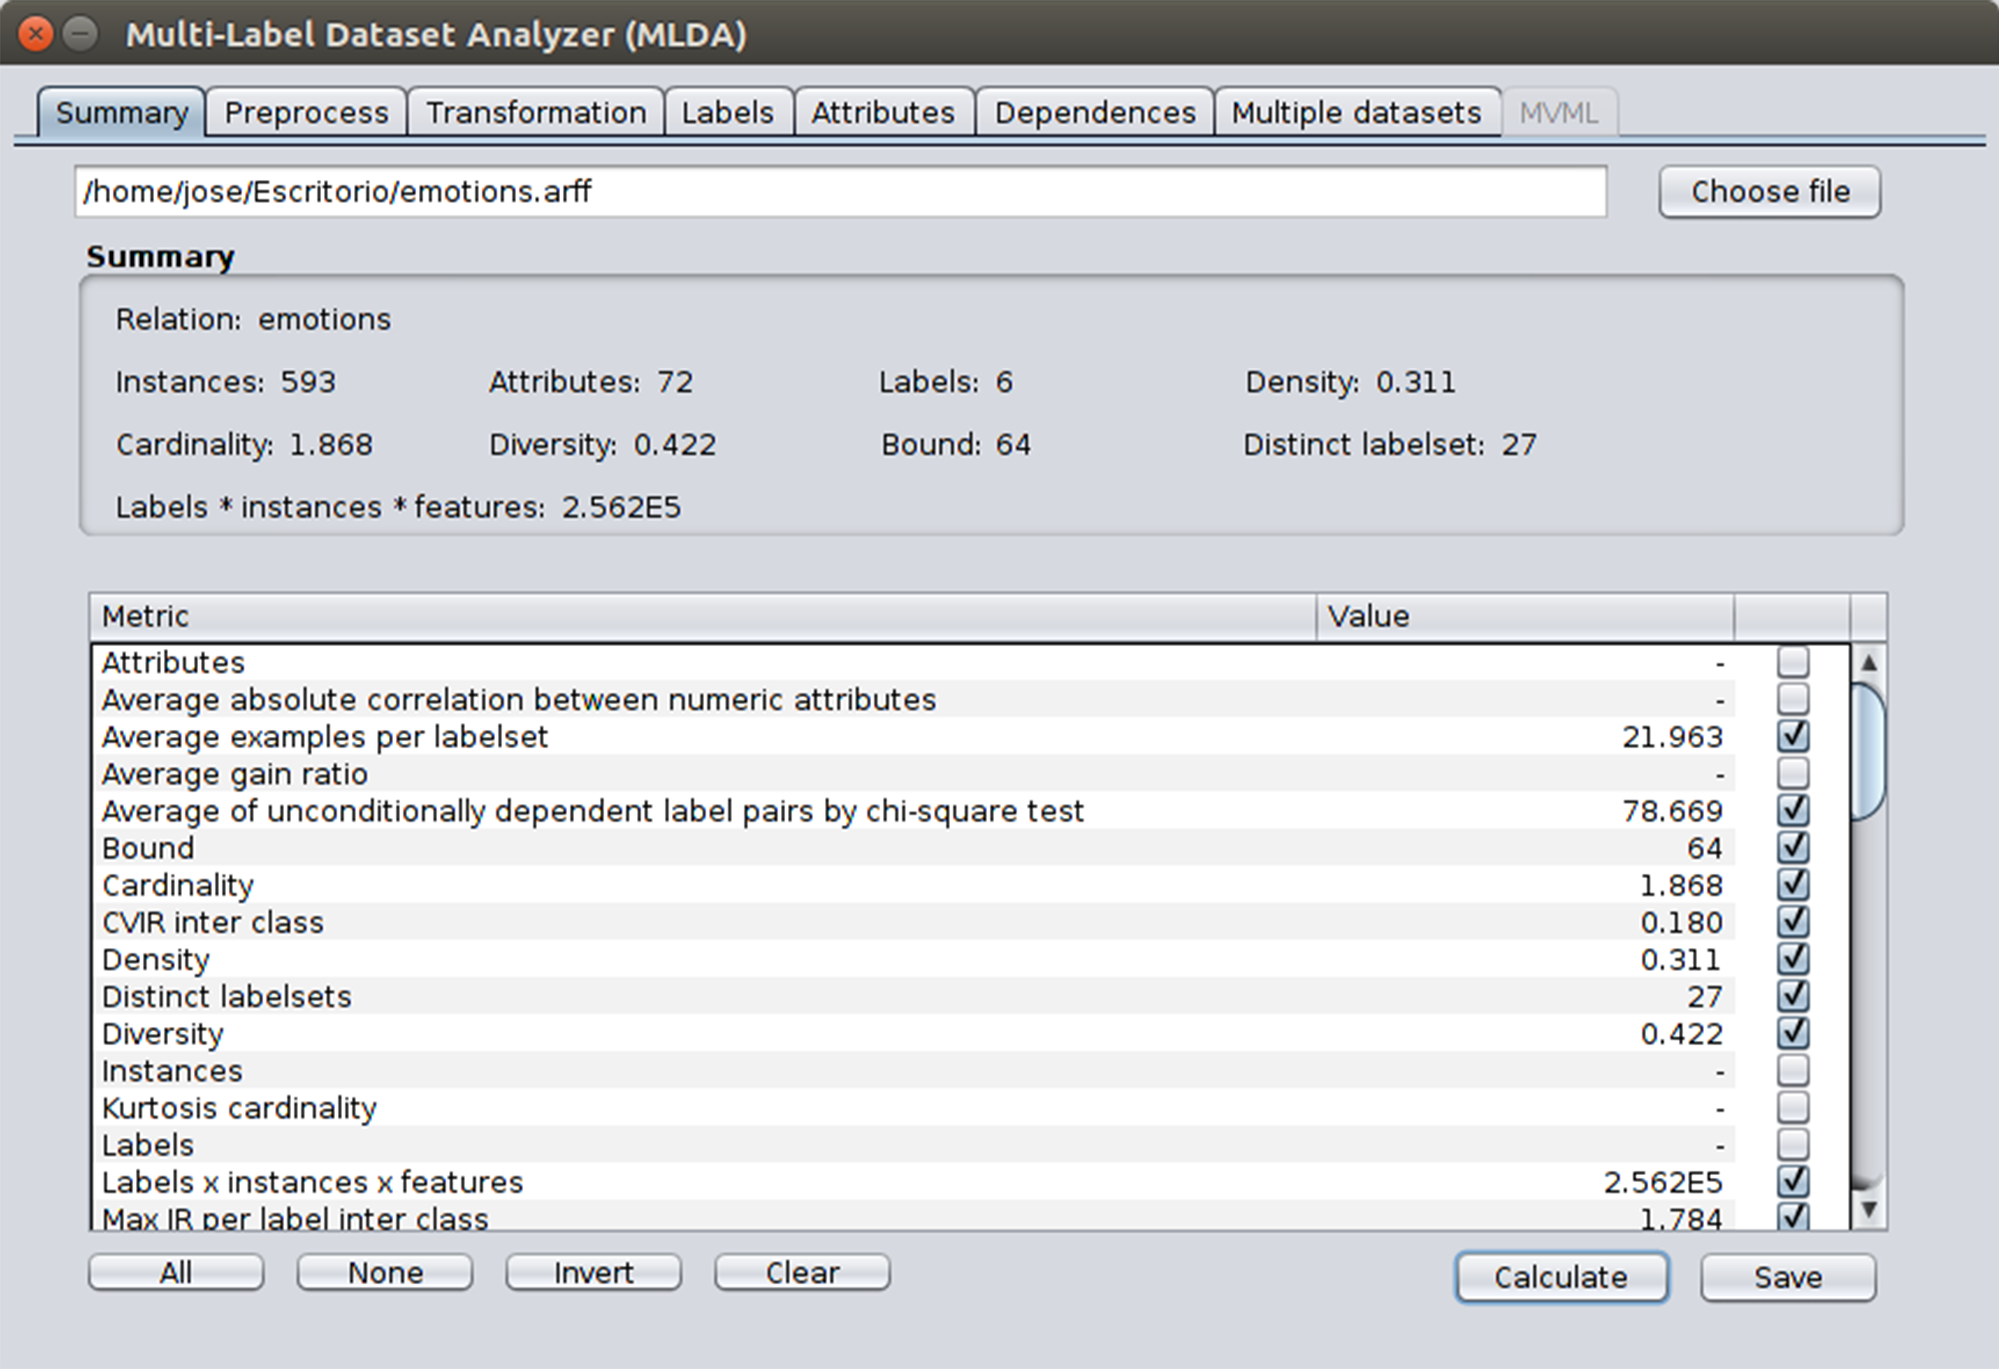
\includegraphics[width=0.5\textwidth]{figs/fig1.png}
  \caption{Mi Figura}
  \label{fig:fig2}
\end{figure}

Utilizando subfiguras.
\begin{figure}[htbp]
\centering
\subfigure[SubF1Caption]{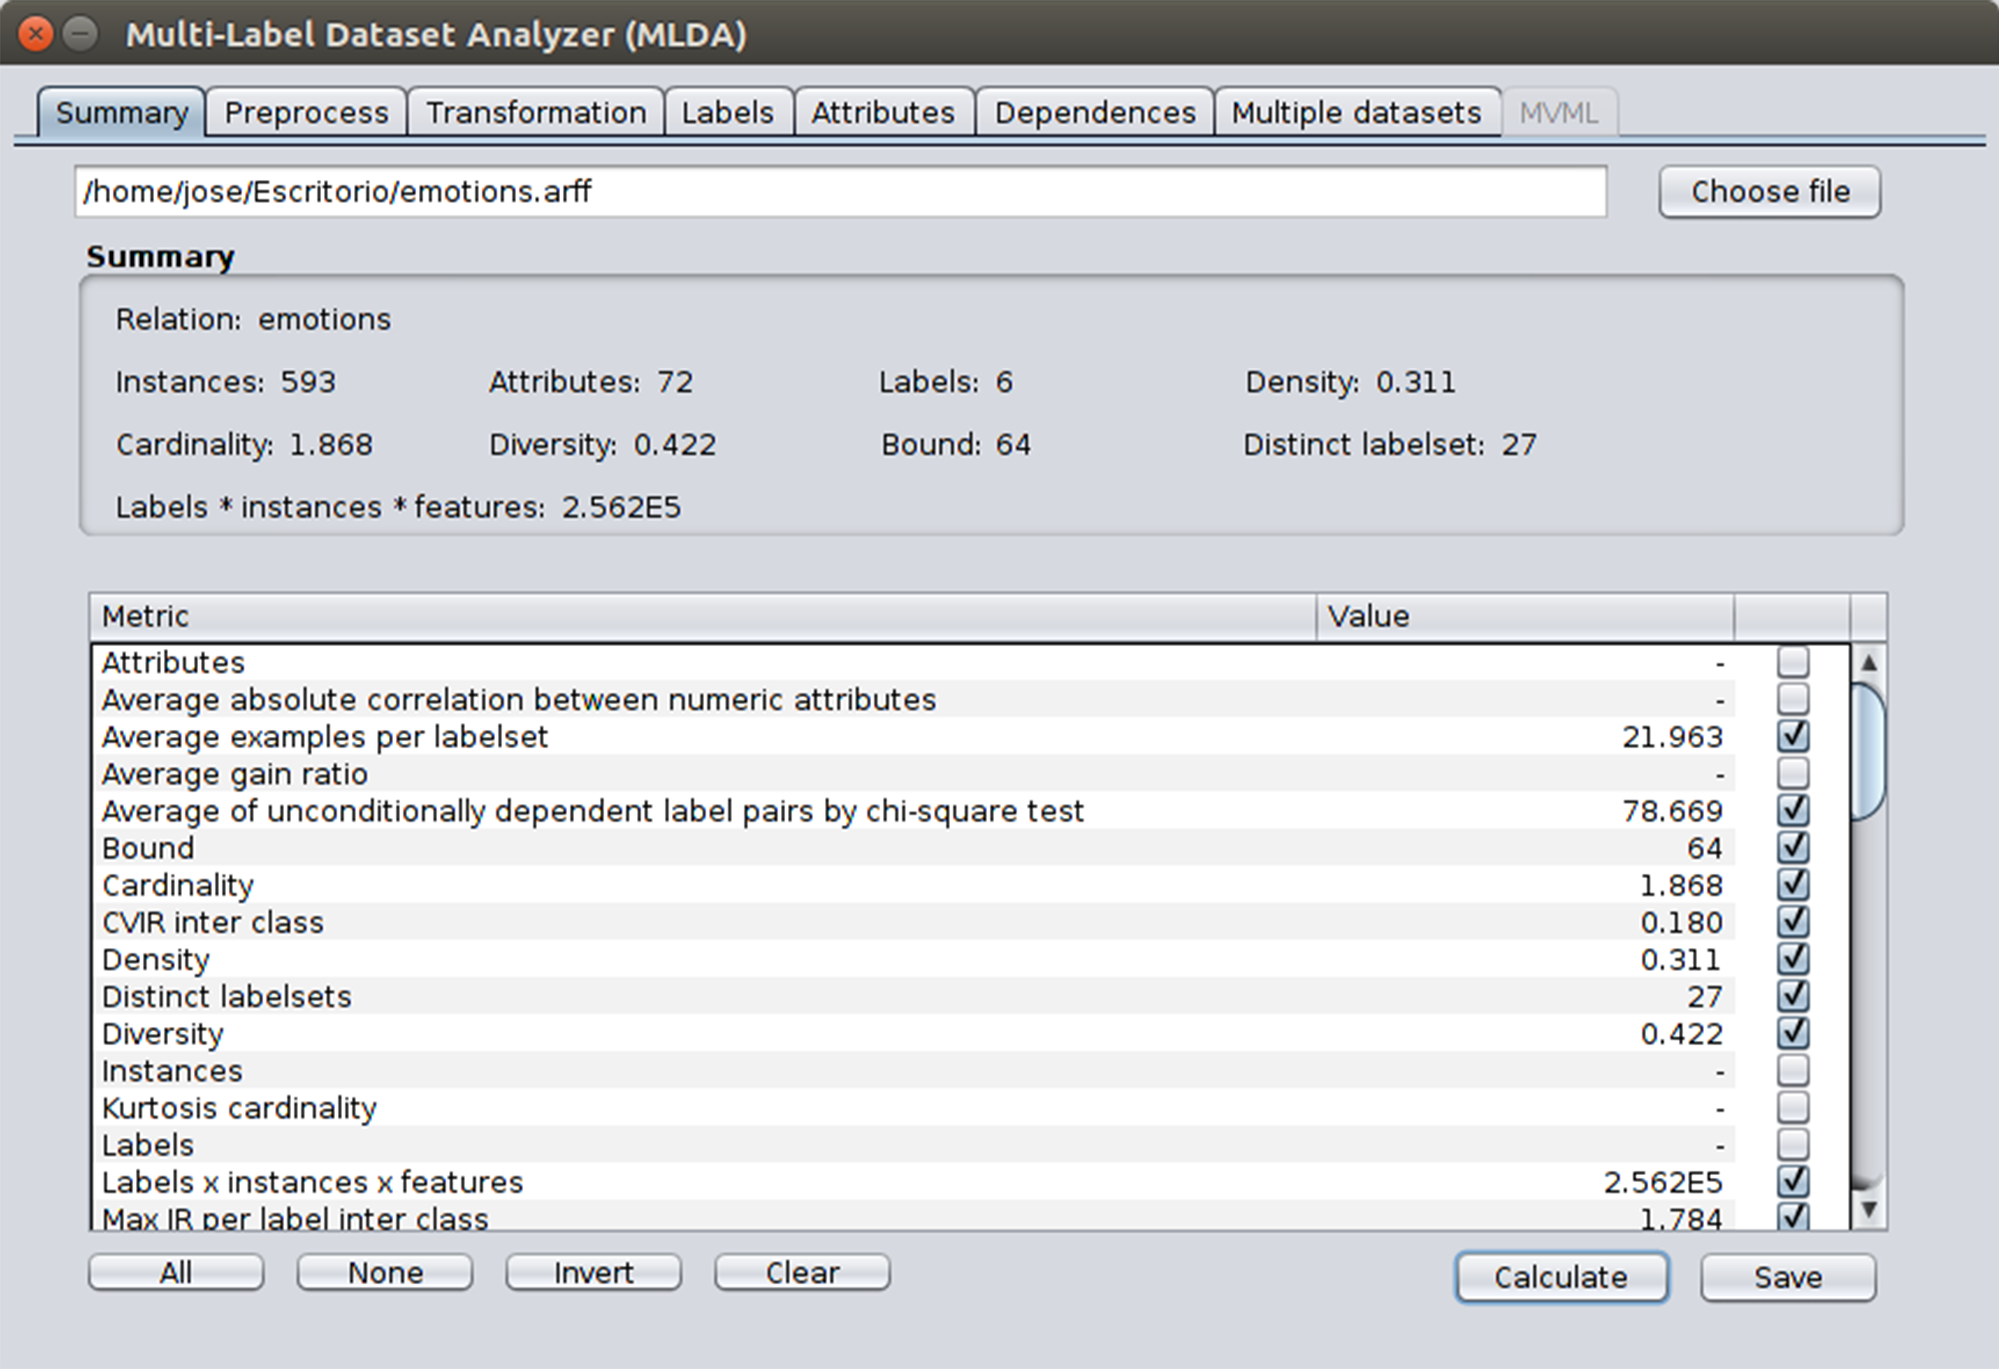
\includegraphics[width=0.45\textwidth]{figs/fig1.png}}
\subfigure[SubF2Caption]{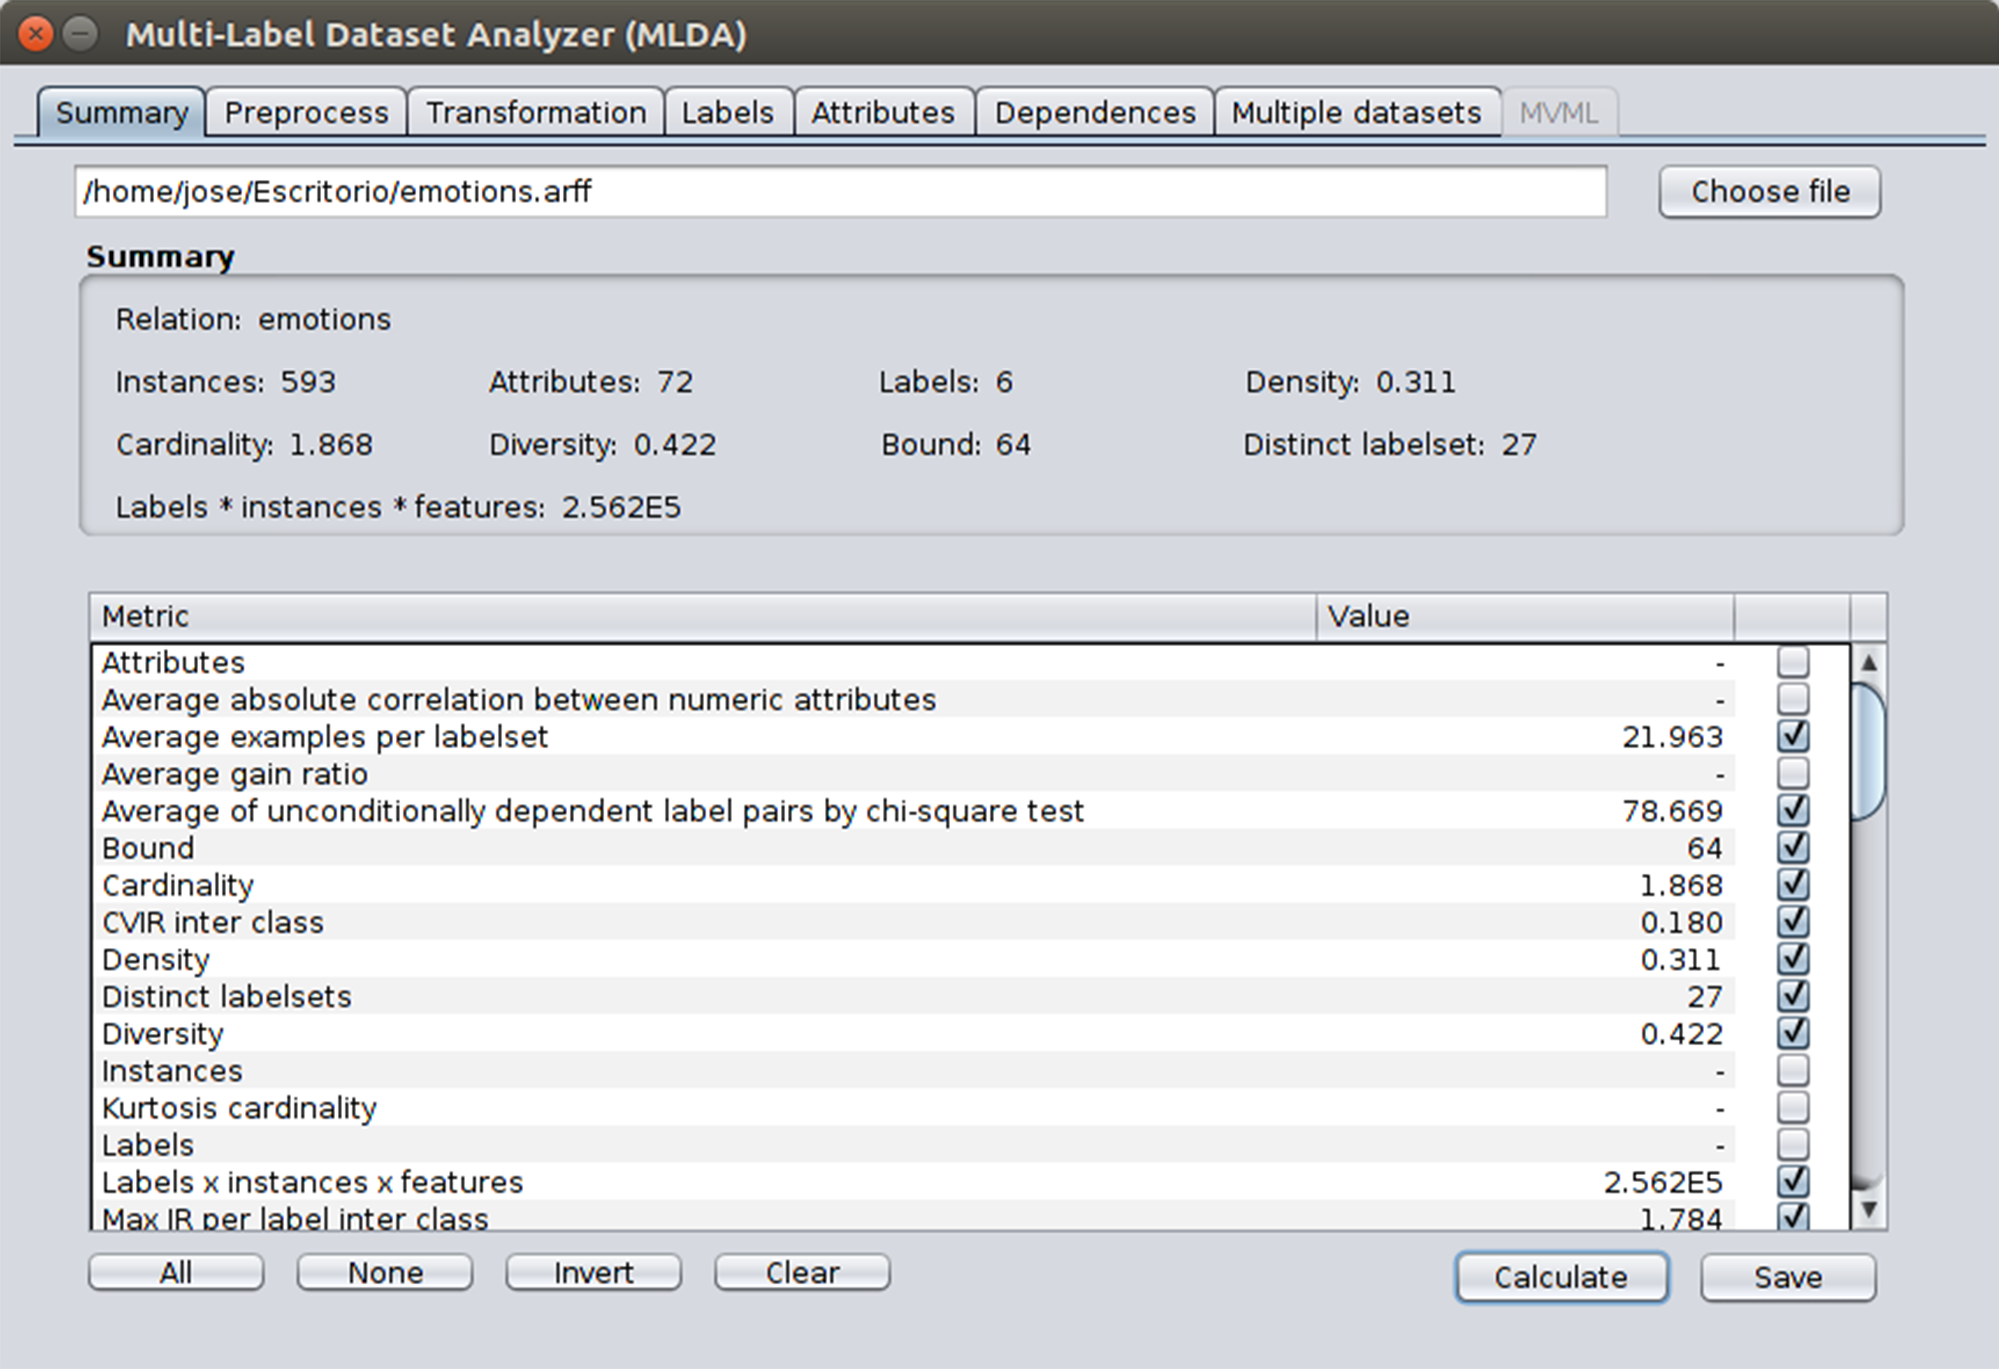
\includegraphics[width=0.45\textwidth]{figs/fig1.png}} \\
\subfigure[SubF3Caption]{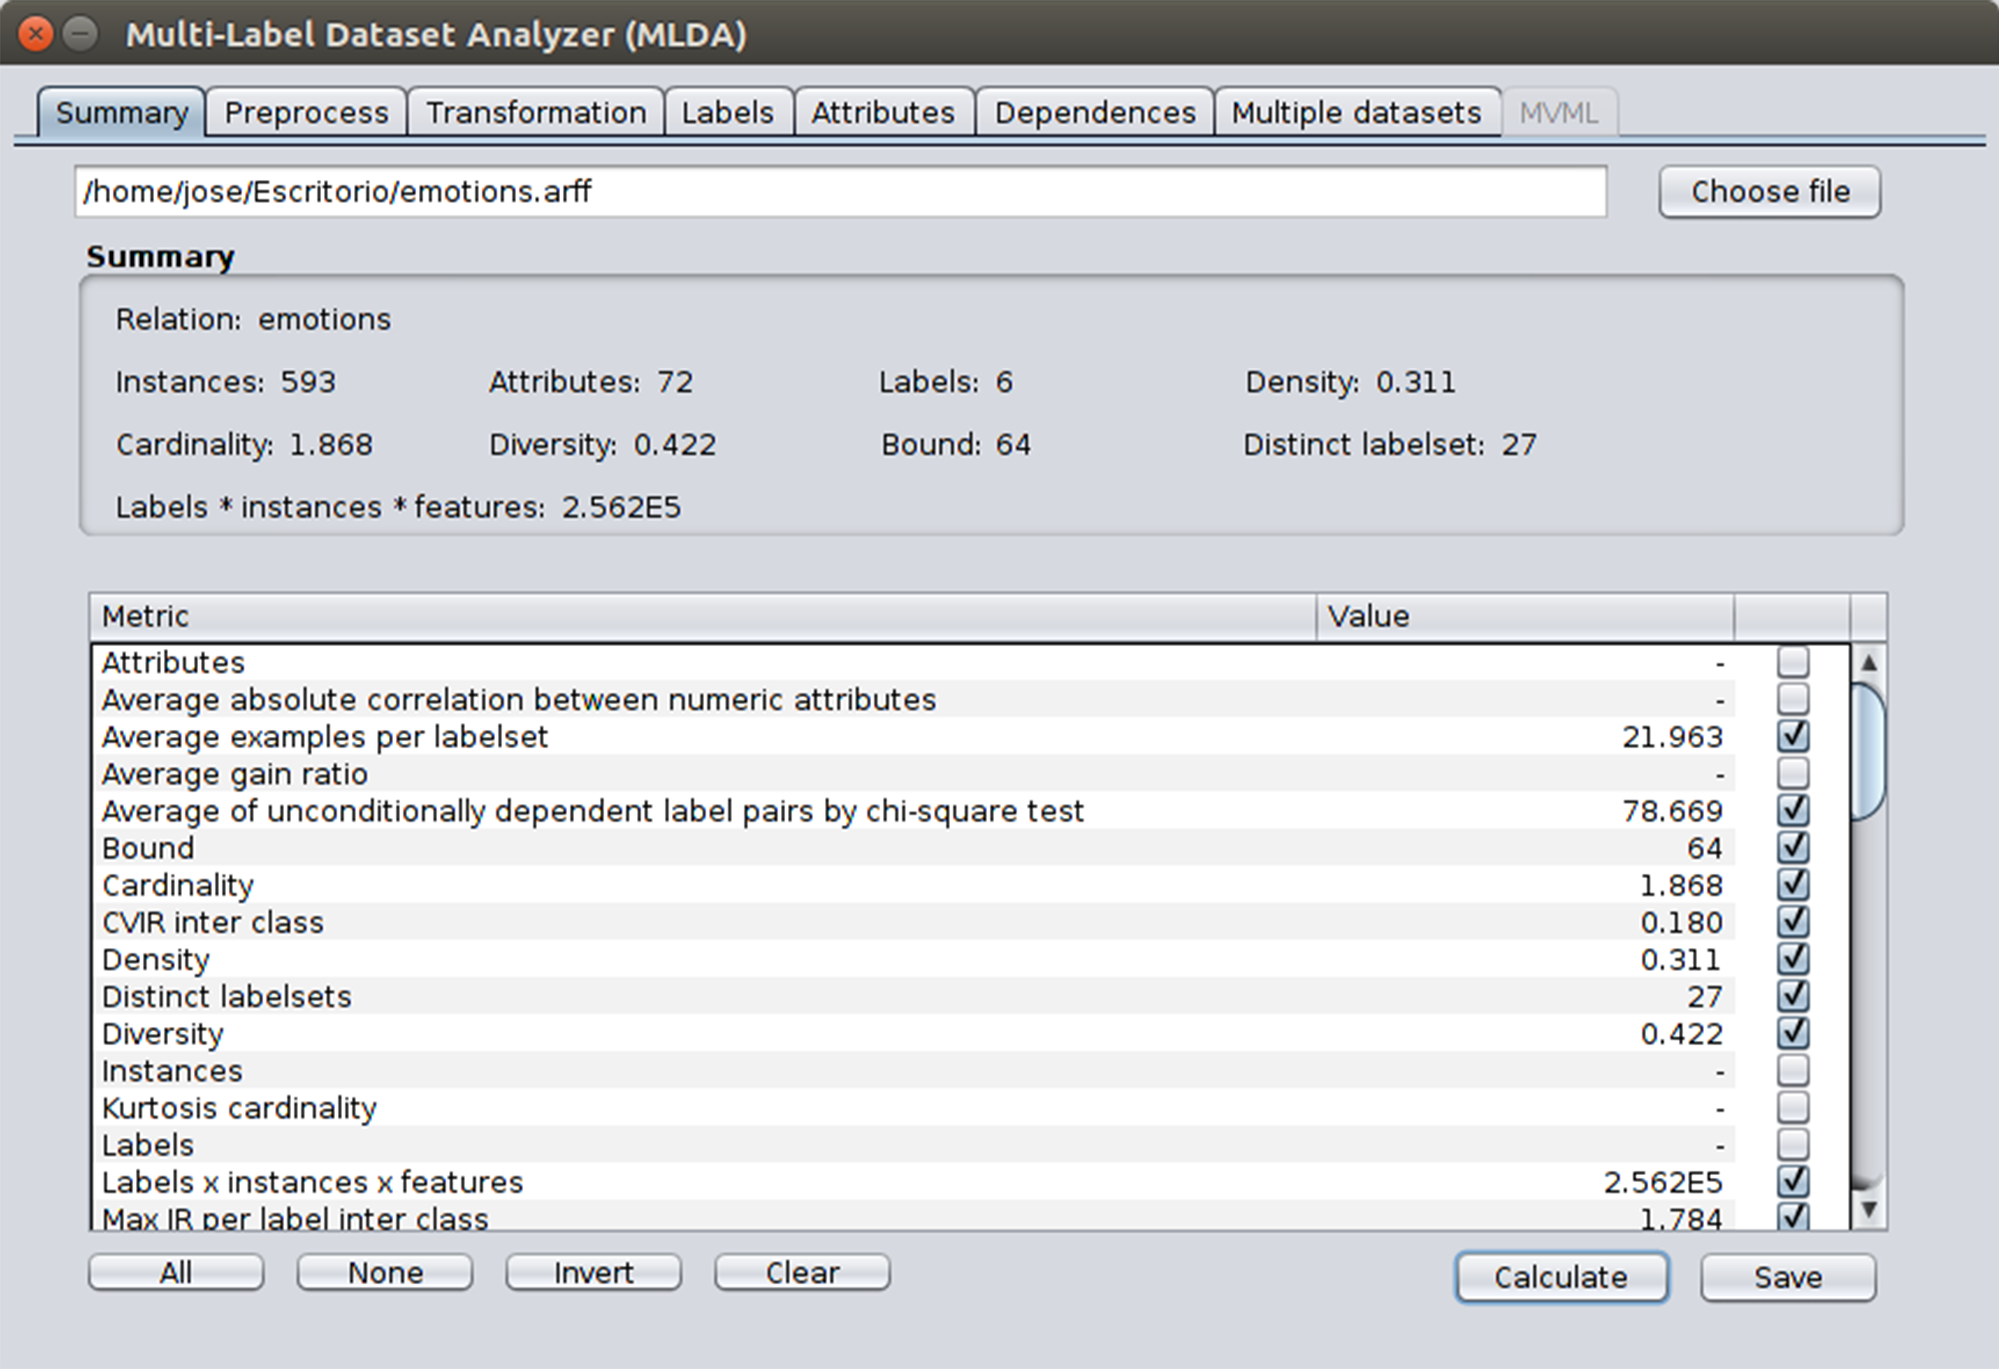
\includegraphics[width=0.45\textwidth]{figs/fig1.png}}
\caption{Global Caption.} \label{fig:subfigs}
\end{figure}

\end{document}
